% Please do not change the document class
\documentclass{scrartcl}

% Please do not change these packages
\usepackage[hidelinks]{hyperref}
\usepackage[none]{hyphenat}
\usepackage{setspace}
\doublespace

% You may add additional packages here
\usepackage{amsmath}
\usepackage{graphicx} 
\graphicspath{ {Figures/} }

% Please include a clear, concise, and descriptive title
\title{Are User Stories a Suitable Metric for Burn Down Charts in Agile Game Development?}

% Please do not change the subtitle
\subtitle{COMP150 - Agile Essay}

% Please put your student number in the author field
\author{1507866}

\begin{document}
	
\maketitle
	
\abstract{This essay will analyse the use of user stories in burn down charts in the Agile development process. The focus will be on the use of user stories as a metric in burn down charts and they're suited to use in the games industry.}
	
\section{Introduction}

Kupianinen \textit{et al} say that burn down charts are a measure that should be used by Agile teams \cite{Kupiainen}. The intention of this essay is to look at the use of user stories in burn down charts in the Agile and Scrum development processes. It will also look at whether they are suited to use in games development.

\section{What is the Agile philosophy?}

Agile is a software development method that focuses on the quality of software and finding better ways to develop it \cite{AgileManifesto}. Previously a commonly used software development method was the Waterfall model. This was a sequential process that took place over a series of predefined stages. The clear end to a stage meant that measuring progress in this method was easier than with Agile. \cite{Duka}.

Instead of stages Agile is an iterative process. The development takes place over a series of sprints and during each sprint user stories are completed. User stories are short descriptions from the customer's point of view of a feature that needs to be included in the software. This makes measuring progress in an Agile software development project less clear therefore new metrics are needed for Agile as traditional metrics could be used for Agile but may not give useful data \cite{Misra}.
Scrum is a project management method used alongside Agile. Scrum focuses on customer collaboration with its daily scrum meetings. These meetings are used to discuss who is doing what user story and what the customer wants prioritized \cite{Sutherland}.
There are three main roles in Scrum; the Product Owner, the Scrum Master and the development team. \cite{Ktata}

Agile is suited to use in the games industry as it states in the manifesto that it focuses on responding to change over in depth plans \cite{AgileManifesto}.  Over the development process a game is likely to change a lot. Features may be cut, a certain mechanic may not be fun or an issue arises during play testing. All of these could lead to significant changes in the game. With Agile only the relevant user stories would need to be changed instead of reworking a large design document. Scrum is suited to the games industry as it works with Agile. The daily scrums allow people from different departments to communicate daily and ensure everything is going smoothly.
%Needs refs?

\section{Metrics and Burn Down Charts}

Metrics are used to quantify software, this could be measuring the development resources or the development process \cite{Misra}. In this essay measuring will refer to progress made in the development process. 

The metrics used should identify and measure areas that will affect the software \cite{Misra}.
During software development there are many areas that can be measured. However as Hartmann and Dymond point out, just because something can be measured does not mean it should be \cite{Hartmann}.

Burn down charts are a common way to measure Agile software development. They are used to record a chosen metric, such as how many user stories were completed in the last sprint \cite{AgileWithScrum}. Velocity can be used in burn down charts to predict an outcome for the given metric. For example how many sprints it will take to complete the project based on how many user stories have been completed in past sprints. %ref

\begin{figure}[h]
	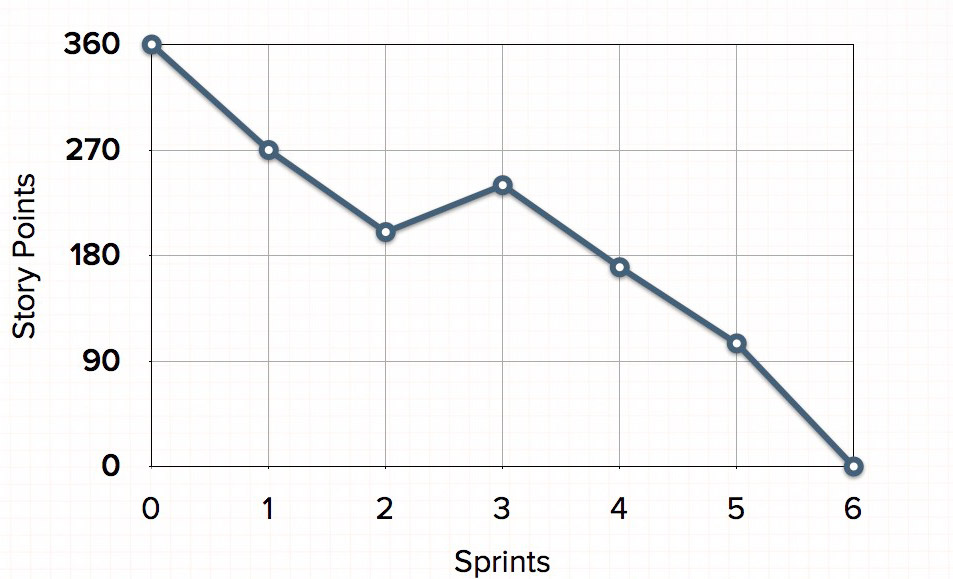
\includegraphics[width=1.0\linewidth]{BDChart.jpg}
	\caption{ An example of a burn down chart \cite{MGS}.}
\end{figure}

Figure 1 above shows an example of a burn down chart. This chart is recording the number of user stories left after each sprint. Velocity could have also been used with this graph to make predictions on how many more sprints would be required to finish all the user stories.


Hartmann and Dymond say that ``measurement drives behaviour "\cite{Hartmann}.  %FIND PAGE!
Therefore the metrics should be designed to shape the software development process. A poorly designed metric will likely give unhelpful data \cite{Ktata}.  Selecting a metric can measure progress but can also aid business decisions and may effect team morale. %FIND REF

There is also the issue of ``vanity vs sanity" metrics. Some metrics may look impressive but not give useful data. For example time, recording how many hours the project was worked on may be a \textit{``vanity"} metric as it may look impressive if the game was worked on for five hundred hours. However that gives no indication of whether all the features have been implemented. An example of a more useful metric may be user stories, this metric can be used to see what features have been implemented or what percentage of the user stories have been completed.

%Different software will likely need different metrics  \cite{Misra}. %CHECK!

User stories are a ....

A simple metric to use in a burn down chart is to record how many user stories are completed in a single sprint. This may work for smaller projects. The issue with this metric is that different user stories may take different amounts of time. Also nearer the end if bugs get put on the backlog this may lead to an invalid velocity. %ref

%Also user stories may not be valid for games development, if there are user stories for each part of the game such as graphics, audio and programming the veloc 

%Using user stories as a metric could be a sufficient way to measure progress in a smaller piece of software. This is because there will be less user stories. In enterprise software most of the user stories will relate to the software again making user stories a more suitable metric. However in games development there will be user stories relating to graphics, audio and many other parts of the game. 

Downey and Sutherland suggest a method where points are assigned to a user story. These points can be based on it's size, importance or the time it'll take to complete \cite{Downey}. Then user stories are chosen based on their points and a baseline velocity for that sprint is calculated from the points. This metric could be suitable for the games industry as it would allow user stories from different parts of the game to be prioritized. ... However an issue with this could be that the importance of a user story could be subjective. 


% TODO:
% Fix focus on question a bit more
% Use a couple more references
% More analysis
% More focus on what makes a metric good?

% Misra - invent the metric as you need it
%	Selecting a metric because it is commonly used may not give useful data
%	- breaks it down to 4 metric types

%Paper 5 - designing agile metrics


\section{Conclusion}
In conclusion ...
% dif software/game etc needs dif metric	
	
\bibliographystyle{ieeetr}
\bibliography{comp150_agile}
	
\end{document}
